\documentclass[PPFS.tex]{template/subfiles}

% \newcommand{\sn}[1]{\textsigfont{\textit{#1}}}
\newcommand{\sn}[1]{\textit{#1}}
\begin{document}
%------------------------------------------
%	SYSTEM ARCHITECTURE
%------------------------------------------
\begin{comment}
    ----- Problem Statement -----
    It is helpful to provide a very simple block diagram of your project very early in the report to provide a
    graphical view that helps the reader understand. This diagram should focus on the interface(s) to your
    project. You may even show your project as a single block. This diagram can be more stylized (perhaps
    with clip art) to get the main idea across to the reader.

    When you get to sections that explain your design process, start with the design of the system
    architecture. This is where you provide a detailed block diagram of your system. Be sure to justify your
    approach. Why did you break down the functionality of the system into the blocks as you did? Were
    there alternative ways to do it?

    In many cases, you may also include a block diagram of the hardware and a separate block diagram of the
    software (and perhaps a system block diagram to show how the two relate). Many teams make the
    mistake of describing the software with very little detail. It is highly recommended that you include a
    block diagram of your software, preferably using the Uniform Modeling Language (UML).
\end{comment}

\section{System Architecture}

% TODO: Create a VERY simple block diagram detailing the entire system.
The system architecture is split into four main categories: Sensors, Displays, Hub, and Server. The overview of the architecture can be seen in \refFig{fig:general_overview}. The system was designed in order to be as low cost as possible, while still retaining generality for many different types of gyms. This architecture attempts to address problems of range, variable amounts of gym equipment and scalability.

\begin{figure}[H]
    \centering
    % A task for another day
    % \includesvg[clean,png,width=5cm]{general_overview}
    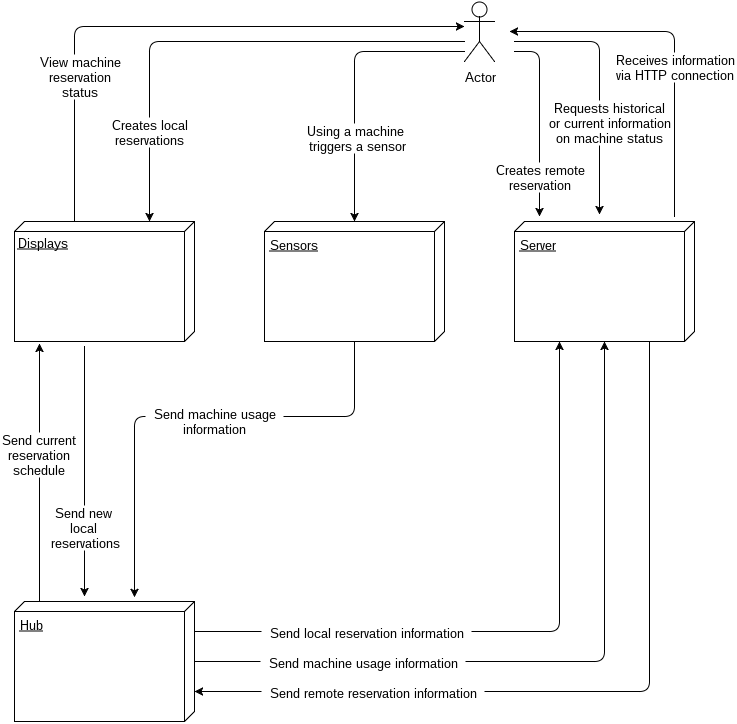
\includegraphics[width=0.75\textwidth]{uml/general_overview.png}
    \caption{UML Diagram of the Sensor Architecture}
    \label{fig:general_overview}
\end{figure}

The displays and sensors would be placed on individual gym equipment, so that the user would have a by-machine understanding of the reservations upcoming for a given machine. The sensors' main goal is to send information back to the hub, for collation by the server. The goal of the hub is to gather the data from the sensors and the display and send it to the server, as well as distribute remote reservation data to the displays. Finally, the server interacts with the user and sends information as requested to the user. It also handles any new reservation requests.

One way the user interacts with the system via HTTP requests to the server, primarily for requesting information or setting reservations. Another way the user will interact with the system is using the gym equipment. By doing so, they will activate the sensors, who will update the hub. The final way the user interacts with the system is by reading from the displays and finding out the information about reservations for that machine.

\subsection{Sensors}

To accomplish the goal of having a sensor network with a wide range, but long battery life, it was decided that a mesh network system would be necessary. In general, to make a signal have a longer range, more power is given to a bigger antenna. This was not an option for sensors where the expected battery life must be greater than one year. However, a small range was not acceptable to fulfill the requirement of a generic system that would fit most any gym, so it was out of the question to settle for a small range. Another option is to use sensors that are capable of communicating to each other and then funneling that information through the other sensors to a centralized hub that would collect this data: a mesh network.

% This is a terrible intro to this
The basic UML diagram in \refFig{fig:sensor_arch} details the connections between the sensors, between the sensor and the hub, and between the sensor and the user.

\begin{figure}[H]
    \centering
    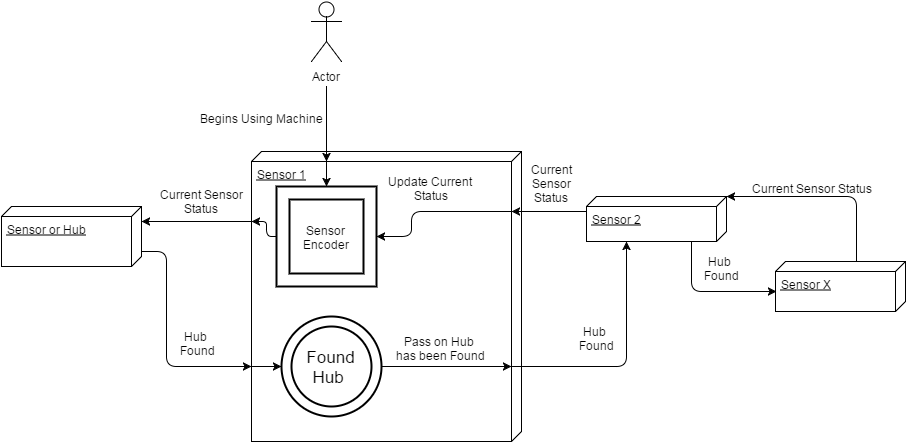
\includegraphics[width=\textwidth]{uml/sensors.png}
    \caption{UML Diagram of the Sensor Architecture}
    \label{fig:sensor_arch}
\end{figure}

The sensor architecture can be thought of as funnel. The further out from the hub a sensor is, the further away it is from the center of the funnel. To communicate with the hub, each sensor will filter its information down to the hub through other, closer, sensors.

To be able to fulfill this design architecture, each sensor will contain two main processes. The first process is \sn{Hub Found}. The \sn{Hub Found} signal will alert other sensors further away from the hub that the destination is "down this way." This will allow sensors, if this attribute is detected, to not continue to search for other devices to make connections to, but to focus on only one (or perhaps two for redundancy's sake) and thus conserve power. The second process is \sn{Sensor Encoder}. This process will encode the information recorded by that sensor can be linked to that sensor. This allows the sensor to pass on useful information about itself,  along with being able to send the data from previous sensors. This ensures that the information is kept separate and particular to each machine. This is integral to determining which machines are in use and maintaining realistic reporting for both real-time and historic services. This process is activated by an outside actor using the equipment.

The information contained in \sn{Current Sensor Status} signal is the encoded data that will -- eventually -- be sent to the hub. After arriving at the hub, that data will be sent to the server for processing.

\subsection{Displays}

The displays are the answer to the problem of showing the user if a machine is reserved or will be reserved shortly. They also will allow the user to create a reservation locally to ensure that they will not be asked to leave the machine before they are ready to leave.

With the need to learn about remote reservations and push local reservations, the displays encountered a similar problem as the sensors: low power and long distance communication. With that similar problem came a similar solution: displays with mesh networking capability. In the \refFig{fig:display_arch}, one can see that the displays are designed to communicate with each other as well as the hub.

\begin{figure}[H]
    \centering
    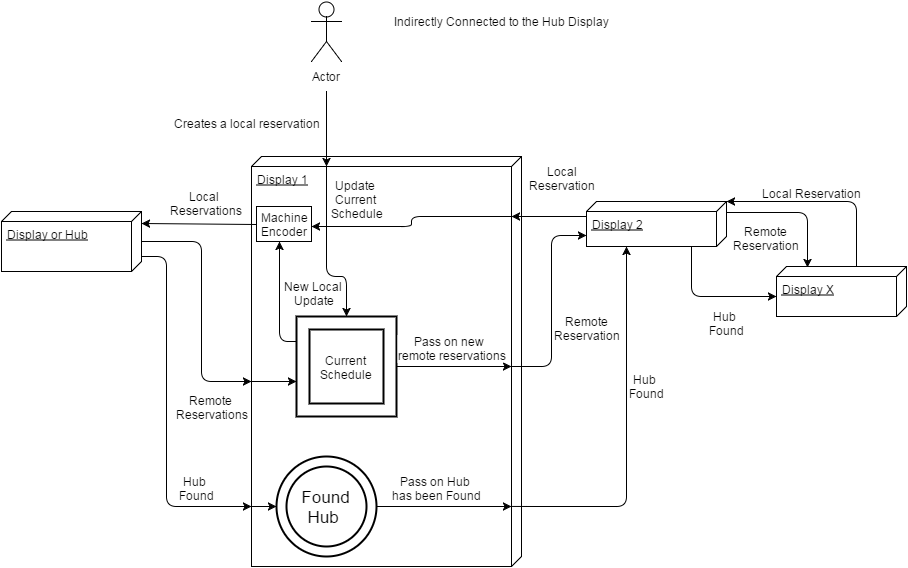
\includegraphics[width=\textwidth]{uml/displays.png}
    \caption{UML Diagram Detailing the Display Architecture}
    \label{fig:display_arch}
\end{figure}

Extending the analogy presented for sensors, the displays will funnel any information about local reservations down to the hub through other display units. They will also pass a \sn{Hub Found} signal up the chain of displays to communicate when searching is not required any longer. However, displays must also retrieve information about remote reservations and thus have an additional connection when compared to the sensors. Due to the three different streams of information, the display contains three distinct entities within itself.

The first entity is the \sn{Hub Found} entity, which completes the same function as the \sn{Hub Found} entity within the sensors. The second entity is the \sn{Current Schedule} entity. This is a basic database that contains all the information regarding the reservation schedule for the current day for this machine. It takes in a remote reservation signal and decides if it is pertinent to this display. If the reservation is pertinent, it updates the \sn{Current Schedule}. If the reservation is not pertinent, it continues sending the encoded information to the next sensor, or "up the funnel." The third entity is the \sn{Machine Encoder}, which will only send information if a local reservation has been initiated by an outside actor. It will also encode any other local reservations made by machines up the funnel and then send that down the funnel. The funnel here being the same type of mesh network that the sensors use, they can be their own network or simply be part the same network as the sensors. This is similar to the encoding of the signal in the sensors to ensure that the data received by the hub can be matched to a specific piece of equipment.

\subsection{Hub}

Now that all the information from the sensors and the displays has been "funneled" into the hub, the hub's first purpose is to transfer this information up to the server for processing. The other purpose is to transfer any new information to the displays, along with transferring the \sn{Hub Found} signal to the displays and sensors directly connected to the hub. This is illustrated in the \refFig{fig:hub_arch}.

\begin{figure}[H]
    \centering
    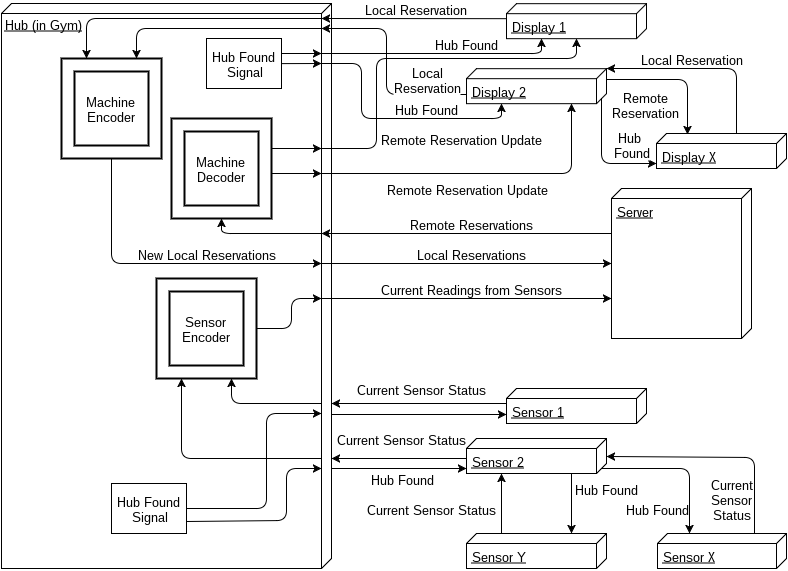
\includegraphics[width=\textwidth]{uml/hub.png}
    \caption{UML Diagram Detailing the Hub Architecture}
    \label{fig:hub_arch}
\end{figure}

The hub has several key processes that affect both the sensors and the displays. It must encode all of the signals that it gets from the sensors into something that it is able to send to the server for the processing of the signals. This will most likely include taking the information and forming a packet that is sent to the server. Because it can connect to several different sensors, it must have its own \sn{Sensor Encoder} that encodes which sensors sent which data into the packet that will be sent to the server. The hub will also send a \sn{Hub Found} signal to any connected sensors to ensure the sensors are funneling their readings to the correct location.

The hub also handles all of the connections from the displays. A \sn{Machine Decoder} is necessary in the hub because it disseminates remote reservation information from the server to the displays. The \sn{Machine Decoder} is where the hub will take the information from the server and decode that data into display-specific data. It also receives information from the displays, so it must have a \sn{Machine Encoder} that takes the information received from the displays about local reservations and then passes that along to the server. After the information is encoded and sent, the server can maintain an up-to-date schedule. Once again, the hub sends a \sn{Hub Found} signal to the displays so that each display can confirm it is sending the data to the correct location.

The hub has three basic types of connections. The first type of connection is when the hub makes a connection to the server which carries information about local reservations made by actors in the gym. The second type of connection is when the sensors create a connection to the hub. On this connection the sensors send information on the current status by sensor. This signal is properly encoded. The third connection is when the hub receives information about remote reservations. This connection provides the information that will later be passed, after decoding, to the displays for up-to-date representation of the current schedules by machine.

\subsection{Server}

The server's main purpose is to track the information both from sensors and from remote users. It will take the information from the sensors, process the data, and then be able to represent what machines are currently in use. It will pass that information to three primary locations: \sn{Current Reservation Database}, \sn{Historical Use Database}, and \sn{Current Use Database}.

The \sn{Current Reservation Database} will contain recent reservations made both locally and remotely. Additionally, if a machine is currently in use the entity will prevent someone from reserving that piece of equipment for a set amount of time. This prevents a user from being kicked off a machine unexpectedly. Because of this, the database will be updated from HTTP requests (from the World Wide Web actor), local reservation requests (human actor in the gym), and from current status readings (made by sensors in the gym). The database will forward any new reservations to the machines by sending the information to the hub. The \sn{Current Reservation Database} will contain all the reservations that have not yet been completed for the machines. It was designed as a separate database so that sending information to the machines would be simpler and quicker, as a very large (and ever-growing) database would not have to be queried to send up-to-date information about reservations.

The \sn{Historical Use Database} will exclusively track the information by machine that is received from the hub. It will act as the pool of information that administrators can draw upon to gain insight into the use of the machines and that clients will draw upon to gain health and habit insights on. It is planned to be a log of all past-use by machine. It will also contain information about reservations made, including if they were fulfilled, fulfilled on time, and proportion of time the machine was used with and without reservation.

The \sn{Current Use Database} is a simpler version of the Historical Use Database in that it will not log use of the past machines, but it will keep a record of whether a machine is currently in use or not. This system is shown in \refFig{fig:server_arch}.

\begin{figure}[H]
    \centering
    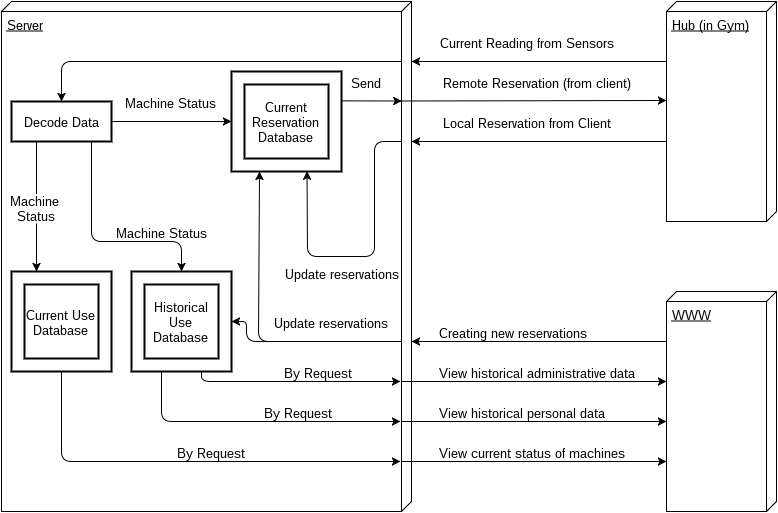
\includegraphics[width=\textwidth]{uml/server.png}
    \caption{UML Diagram Detailing the Server Architecture}
    \label{fig:server_arch}
\end{figure}

The server's main purpose will be to capture and receive the current use from the hub, while sending any remote reservations gained via HTTP requests. It will also log and display current use of the machines for personal and administrative use.

\end{document}
